\documentclass[a4paper, 10pt]{article}

\usepackage[utf8x]{inputenc}
\usepackage[english, russian, ukrainian]{babel}
\usepackage{cmap}

\usepackage{graphicx}
\usepackage{float}
\usepackage{multicol}
\usepackage{multirow}
\usepackage{amsmath}

\usepackage{geometry}
\geometry{top = 2cm}
\geometry{bottom = 2cm}
\geometry{left = 3cm}
\geometry{right = 1.5cm}

\begin{document}
\begin{titlepage}
\begin{center}
\large{
Міністерство освіти і науки, молоді та спорту України\\
Національний технічний університет України\\
``Київський політехнічний інститут''\\
Факультет прикладної математики\\
Кафедра спеціалізованих комп’ютерних систем\\
}

\vfill

\large{\bf{
Лабораторна робота №1\\
Дисципліна:\\
``Архітектура комп'ютерів''\\
Тема:\\
``Арифметико--логічні пристрої з розподіленою логікою''\\
}}

\vfill

\begin{table}[h]
\centering
\begin{tabular}{lp{4cm}l}
Виконав:&&Перевірив:\\
Студент групи КВ--92&&Жабін В. І.\\
Гуль О. В.&&\\
Залікова книжка № КВ--9203&&\\
\end{tabular}
\end{table}

\vfill

Київ \the\year
\end{center}
\end{titlepage}
\newpage

\section{Мета}
Одержати навички в проектуванні арифметико--логічних пристроїв з розподіленою логікою і автоматів управління з жорсткою логікою.

\section{Завдання}
\begin{enumerate}
    \item Варіанти завдання визначаються молодшими розрядами $a_{7},\cdots,a_{1}$ двійкового номера залікової книжки.
    \item Розробити структурну схему операційного пристрою та змістовний мікроалгоритм обробки  додатних чисел відповідно до завдання наведеного у табл. 2.7. Для побудови схеми використати комбінаційний суматор, регістр--лічильник циклів та асинхронні регістри, що мають входи управління зсувами і занесенням інформації. На схемі повинні бути зазначені розрядність регістрів та шин.
    \item Розробити функціональну схему операційного пристрою.
    \item Виконати логічне моделювання роботи операційного пристрою за допомогою цифрової діаграми  із зазначеними викладачем значеннями операндів.
    \item Здійснити синтез пристрою управління, тип управляючого автомату обрати із табл. 2.9. Пам’ять автомата реалізувати на тригерах, тип яких обрати з табл. 2.8. Ураховувати, що мікрооперації на регістрах виконуються за перепадом управляючих сигналів з 1 в 0.
    \item Побудувати часові діаграми роботи автомата для кожної комбінацій значень логічних умов.
\end{enumerate}
Варіант: $9203=10001111110011_2$.\\
$a_{7},\cdots,a_{1}=1110011.$\\
Функція: $D=A(B+1)+0.5C.$\\
Тип автомата: Мура.\\
Тип тригера: T.\\
Ураховувати, що мікрооперації на регістрах виконуються за перепадом управляючих сигналів з 1 в 0.

\section{Теоретичні відомості}
Синтез арифметико--логічних пристроїв з розподіленою логікою.\\
За структурою розрізняють АЛП з розподіленою та зосередженою логікою (інакше АЛП із закріпленими та загальними мікроопераціями).
В АЛП першого типу апаратура для реалізації мікрооперацій розподілена між регістрами та закріплена за ними, тобто кожен регістр використовує власну логіку для виконання мікрооперацій. У пристроях другого типу всі логічні ланцюги об'єднані в арифметико--логічному блоці, а всі регістри реалізовані у вигляді надоперативного запам'ятовуючого пристрою.
АЛП з розподіленою логікою складаються з двох функціональних частин: управляючий пристрій, що забезпечує формування всіх управляючих сигналів; операційний пристрій, забезпечує перетворення інформації та виконує мікрооперації над машинними словами.
Побудова таких АЛП відбувається за наступними етапами:
\begin{enumerate}
    \item Для кожної операції будується операційна схема та функціональний мікроалгоритм (Ф--мікроалгоритм). Рекомендується обирати такі мікроалгоритми виконання операцій, що краще сполучаються, тобто вимагають однакового напрямку зсувів в регістрах, однакову розрядність регістрів, одні й ті самі джерела операндів суматорів і таке інше.
    \item Обирається розрядність регістрів, лічильників. Виконується логічне моделювання роботи ОПр, наприклад, із застосуванням діаграми стану регістрів при виконанні МА з критичними значеннями операндів.
    \item Розробляється функціональна та принципова схеми ОПр із зазначенням управляючих сигналів для кожного вузла пристрою.
    \item Складається закодований структурний мікро алгоритм (С--мікроалгоритм) виконання заданих операцій.
    \item Виконується синтез управляючого пристрою.
    \item Складається функціональна та принципова схеми АЛП.
\end{enumerate}

\section{Порядок виконання роботи}
\begin{enumerate}
    \item В моделюючій програмі ПРОГМОЛС 2.0 побудувати схему операційного пристрою для множення чисел та доповнити її схемою управляючого автомата. На першому етапі виходи автомата до входів операційного пристрою не підключати. Налагодити окремо схему операційного пристрою та схему управляючого автомата в синхронному режимі. Опис програмного комплексу ПРОГМОЛС 2.0 наведений у додатку М.
    \item Підключити до управляючих входів операційного пристрою виходи автомата. Зробити комплексне налагодження схеми в синхронному режимі й переконатися в правильності одержання результату.
    \item Перейти до асинхронного моделювання. Дослідити зазначені викладачем часові параметри схеми.
\end{enumerate}

\section{Виконання завдання}
Нехай $n=4$. $D=A(B+1)+0.5C$.\\
RGD~-- регістр результату (накопичувач).\\
RGA~-- регістр операнду A.\\
RGB~-- регістр операнду B. Лічильник, формує ознаку Z.\\
RGC~-- регістр операнду C. Реалізує МО зсуву вправо.\\
SM~-- комбінаційний суматор.
\begin{figure}[h!]
\begin{center}
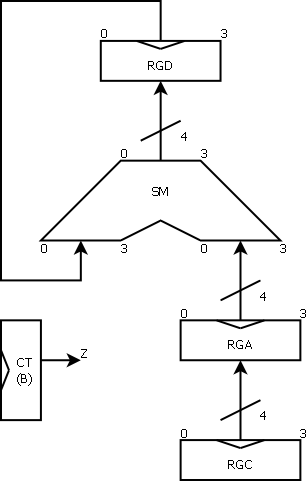
\includegraphics[scale=0.5]{od.png}
\caption{Схема операційного пристрою.}
\end{center}
\end{figure}

\begin{figure}[H]
\begin{center}
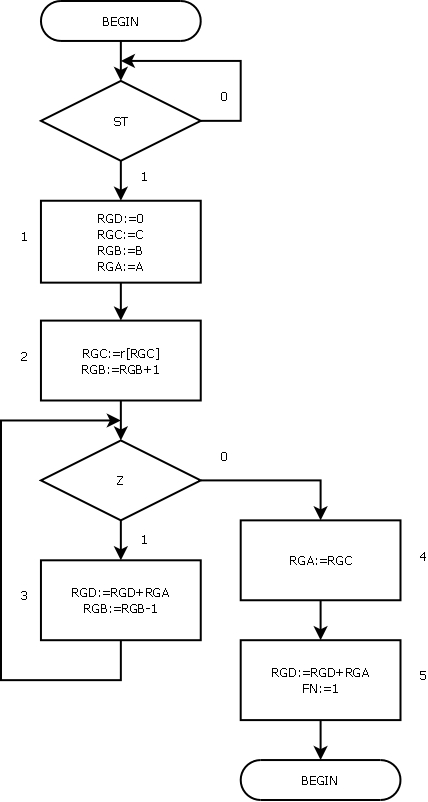
\includegraphics[scale=0.25]{f_alg.png}
\caption{Функціональний мікроалгоритм.}
\end{center}
\end{figure}

\noindent
$A=2=0010_{2}$\\
$B=3=0011_{2}$\\
$C=4=0100_{2}$\\
$D=2(3+1)+0.5*4=10.$
\begin{table}[h!]
\centering
\begin{tabular}{|c|c|c|c|c|}
\hline
 RGA& RGB& RGC& RGD& №MO\\
\hline
0010&0011&0100&0000&1\\
    &0100&0010&    &2\\
    &0011&    &0010&3\\
    &0010&    &0100&3\\
    &0001&    &0110&3\\
    &0000&    &1000&3\\
0010&    &    &    &4\\
    &    &    &1010&5\\
\hline
\end{tabular}
\caption{Дiаграма станiв регiстрiв при виконаннi алгоритму.}
\end{table}

\begin{table}[h!]
\centering
\begin{tabular}{|c|c|c|}
\hline
Елемент & Мікрооперація & Управляючий сигнал\\
\hline
RGA & Запис & W $1\to0$ \\
\hline
RGB & Запис & W $1\to0$ \\
RGB & Інкремент & $+1$ $1\to0$ \\
RGB & Декремент & $-1$ $1\to0$ \\
\hline
RGС & Запис & W $1\to0$ \\
RGС & Зсув вправо & SR $1\to0$ \\
\hline
RGD & Запис & W $1\to0$ \\
RGС & Скидання & R $1\to0$ \\
\hline
\end{tabular}
\caption{Перелік управляючих сигналів елементів.}
\end{table}

\begin{figure}[H]
\begin{center}
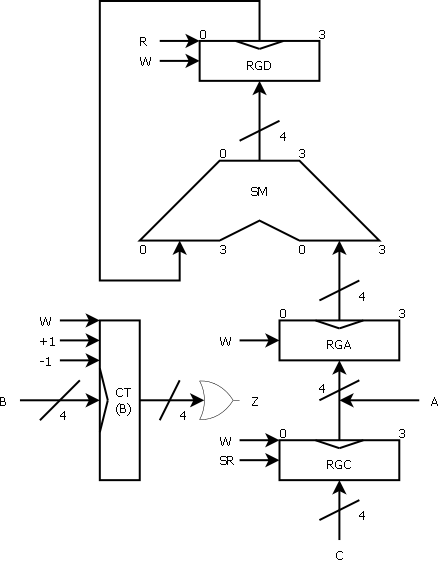
\includegraphics[scale=0.5]{fs.png}
\caption{Функціональна схема операційного пристрою.}
\end{center}
\end{figure}

\begin{figure}[h!]
\begin{center}
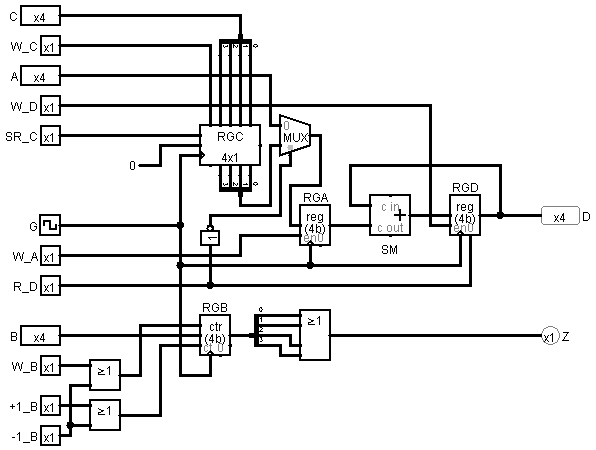
\includegraphics[scale=0.5]{od_circ.png}
\caption{Побудована функціональна схема операційного пристрою.}
\end{center}
\end{figure}


\begin{figure}[H]
\begin{center}
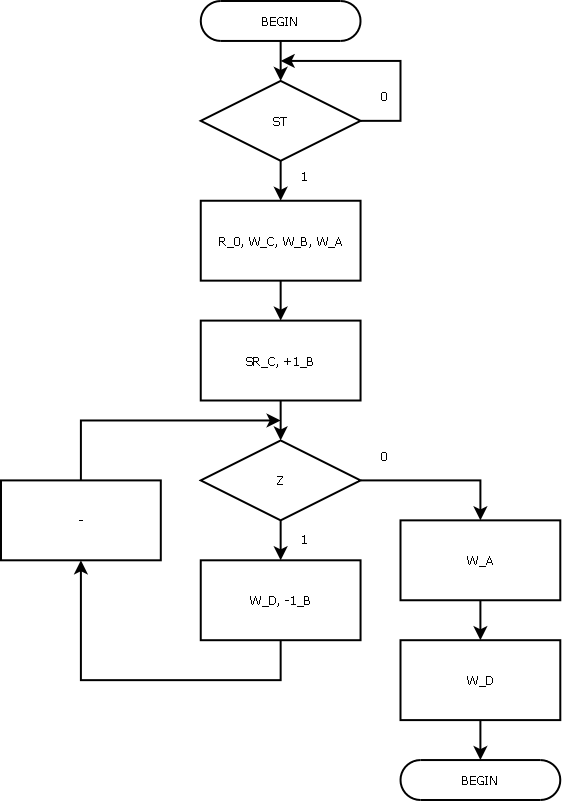
\includegraphics[scale=0.25]{fs_alg.png}
\caption{Функціонально--структурний мікроалгоритм.}
\end{center}
\end{figure}

\begin{table}[h!]
\centering
\begin{tabular}{|c|c|}
\hline
№МО & Мікрооперації та їз код\\
\hline
1 & ($R_D, W_C, W_B$)~-- $Y_1$, ($W_A$)~-- $Y_2$\\
\hline
2 & ($SR_C, +1_B$)~-- $Y_3$\\
\hline
3 & ($W_D$)~-- $Y_4$, ($-1_B$)~-- $Y_5$\\
\hline
4 & ($W_A$)~-- $Y_2$\\
\hline
5 & ($W_D$)~-- $Y_4$, ($FN$)~-- $Y_7$\\
\hline
\end{tabular}
\caption{Кодування сигналів управління.}
\end{table}

\begin{table}[h!]
\centering
\begin{tabular}{|c|c|}
\hline
Умова & Код\\
\hline
Пуск & ST \\
\hline
Кінець & FN\\
\hline
Ненульовий вміст лічильника RGB & Z\\
\hline
\end{tabular}
\caption{Кодування логічних умов.}
\end{table}

\begin{figure}[H]
\begin{center}
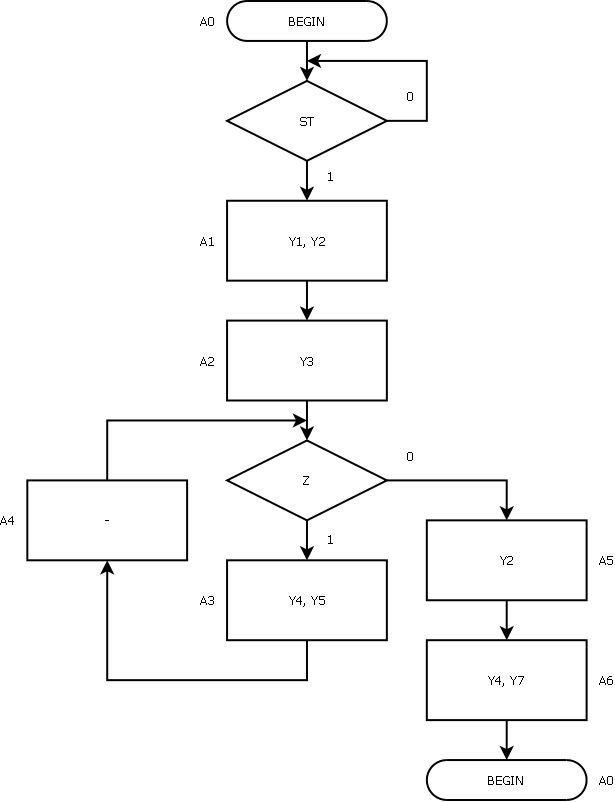
\includegraphics[scale=0.25]{fsz_alg.png}
\caption{Закодований функціонально--структурний мікроалгоритм.}
\end{center}
\end{figure}

\begin{figure}[H]
\begin{center}
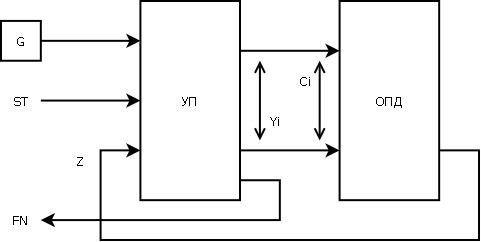
\includegraphics[scale=0.5]{general.png}
\caption{Узагальнена структурна схема АЛП.}
\end{center}
\end{figure}

\begin{figure}[H]
\begin{center}
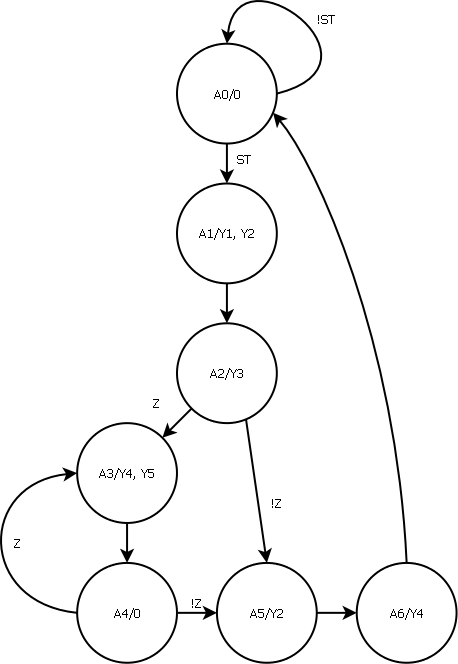
\includegraphics[scale=0.5]{states.png}
\caption{Граф автомата.}
\end{center}
\end{figure}

Всього 7 станів~-- потрібно 3 тригери.
\begin{table}[h!]
\centering
\begin{tabular}{|c|c|c|c|}
\hline
Стан & $Q_2$ & $Q_1$ & $Q_0$ \\
\hline
$A_0$ & 0 & 0 & 0 \\
\hline
$A_1$ & 0 & 0 & 1 \\
\hline
$A_2$ & 0 & 1 & 0 \\
\hline
$A_3$ & 0 & 1 & 1 \\
\hline
$A_4$ & 1 & 0 & 0 \\
\hline
$A_5$ & 1 & 0 & 1 \\
\hline
$A_6$ & 1 & 1 & 0 \\
\hline
\end{tabular}
\caption{Кодування станів автомата.}
\end{table}

\begin{table}[H]
\centering
{\small
\begin{tabular}{|c||c|c|c||c||c|c|c||c|c||c|c|c|c|c|c||c|c|l|}
\hline
\multirow{2}{*}{ПС} &
\multicolumn{3}{|c||}{Код ПС} &
\multirow{2}{*}{НС} &
\multicolumn{3}{|c||}{Код НС} &
\multicolumn{2}{|c||}{Лог. умови} &
\multicolumn{6}{|c||}{Керуючі сигнали} &
\multicolumn{3}{|c|}{Ф--ції збудження} \\
\cline{2-4} \cline{6-19}
  & $Q_2$ & $Q_1$ & $Q_0$ & & $Q_2$ & $Q_1$ & $Q_0$ & ST & Z & $Y_1$ & $Y_2$ & $Y_3$ & $Y_4$ & $Y_5$ & $Y_7$ & $T_2$ & $T_1$ & $T_0$ \\
\hline
\hline
$A_0$ & 0 & 0 & 0 & $A_0$ & 0 & 0 & 0 & 0 & * & 0 & 0 & 0 & 0 & 0 & 0 & 0 & 0 & 0 \\
\hline
$A_0$ & 0 & 0 & 0 & $A_1$ & 0 & 0 & 1 & 1 & * & 1 & 1 & 0 & 0 & 0 & 0 & 0 & 0 & 1 \\
\hline
$A_1$ & 0 & 0 & 1 & $A_2$ & 0 & 1 & 0 & * & * & 0 & 0 & 1 & 0 & 0 & 0 & 0 & 1 & 1 \\
\hline
$A_2$ & 0 & 1 & 0 & $A_3$ & 0 & 1 & 1 & * & 1 & 0 & 0 & 0 & 1 & 1 & 0 & 0 & 0 & 1 \\
\hline
$A_2$ & 0 & 1 & 0 & $A_5$ & 1 & 0 & 1 & * & 0 & 0 & 1 & 0 & 0 & 0 & 0 & 1 & 1 & 1 \\
\hline
$A_3$ & 0 & 1 & 1 & $A_4$ & 1 & 0 & 0 & * & * & 0 & 0 & 0 & 0 & 0 & 0 & 1 & 1 & 1 \\
\hline
$A_4$ & 1 & 0 & 0 & $A_3$ & 0 & 1 & 1 & * & 1 & 0 & 0 & 0 & 1 & 1 & 0 & 1 & 1 & 1 \\
\hline
$A_4$ & 1 & 0 & 0 & $A_5$ & 1 & 0 & 1 & * & 0 & 0 & 1 & 0 & 0 & 0 & 0 & 0 & 0 & 1 \\
\hline
$A_5$ & 1 & 0 & 1 & $A_6$ & 1 & 1 & 0 & * & * & 0 & 0 & 0 & 1 & 0 & 1 & 0 & 1 & 1 \\
\hline
$A_6$ & 1 & 1 & 0 & $A_0$ & 0 & 0 & 0 & * & * & 0 & 0 & 0 & 0 & 0 & 0 & 1 & 1 & 0 \\
\hline
\end{tabular}
}
\caption{Структурна таблиця автомата.}
\end{table}

\begin{eqnarray*}
Y_1&=&Q_0\ \overline{Q_1}\ \overline{Q_2}\\
Y_2&=&Q_0\ \overline{Q_1}\\
Y_3&=&\overline{Q_0}\ Q_1\ \overline{Q_2}\\
Y_4&=&Q_0\ Q_1\ \overline{Q_2} \vee \overline{Q_0}\ Q_1\ Q_2\\
Y_5&=&Q_0\ Q_1\ \overline{Q_2}\\
Y_7&=&\overline{Q_0}\ Q_1\ Q_2\\
T_2&=&\overline{Q_0}\ Q_1\ \overline{Q_2}\ \overline{Z} \vee Q_0\ Q_1\ \overline{Q_2} \vee \overline{Q_0}\ \overline{Q_1}\ Q_2\ Z \vee \overline{Q_0}\ Q_1\ Q_2 =\\
   &=&\overline{Q_0}\ Q_1\ (\overline{Z} \vee Q_2) \vee Q_0\ Q_1\ \overline{Q_2} \vee \overline{Q_0}\ \overline{Q_1}\ Q_2\ Z=\\
   &=&\overline{Q_0}\ Q_1\ \overline{Z} \vee \overline{Q_0}\ Q_1\ Q_2 \vee Q_0\ Q_1\ \overline{Q_2} \vee \overline{Q_0}\ \overline{Q_1}\ Q_2\ Z\\
T_1&=&\overline{\overline{Q_0}\ \overline{Q_1}\ \overline{Q_2} \vee \overline{Q_0}\ Q_1\ \overline{Q_2}\ Z \vee \overline{Q_0}\ \overline{Q_1}\ Q_2\ \overline{Z}} =\\
   &=&\overline{\overline{Q_0} (\overline{Q_1}\ \overline{Q_2} \vee \overline{Q_2}\ Z \vee \overline{Q_1}\ \overline{Z})}\\
T_0&=&\overline{\overline{Q_0}\ \overline{Q_1}\ \overline{Q_2}\ \overline{ST} \vee \overline{Q_0}\ Q_1\ Q_2}\\
\end{eqnarray*}

\begin{figure}[H]
\begin{center}
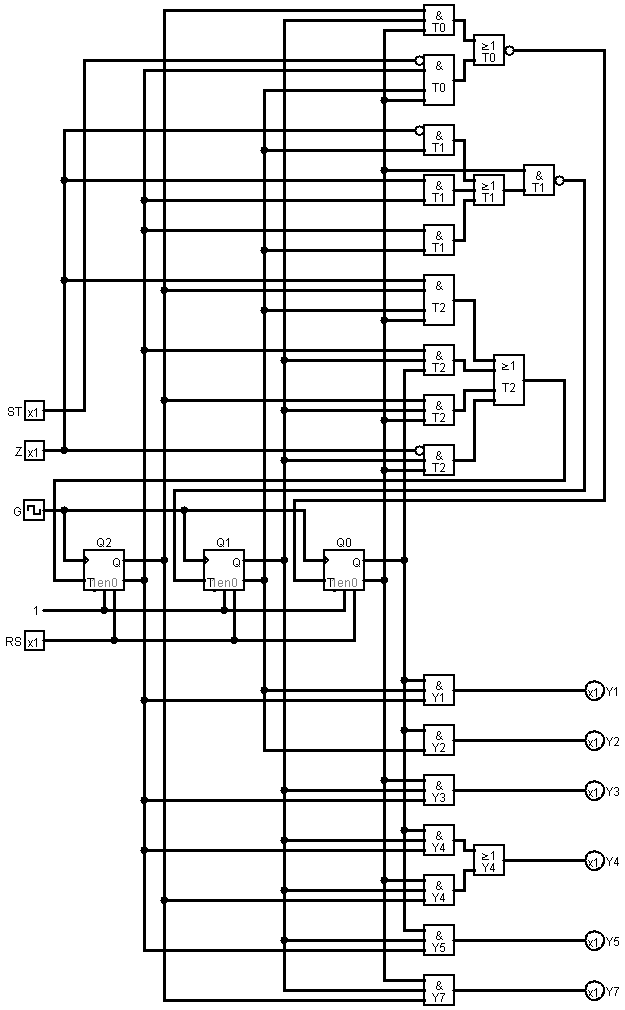
\includegraphics[scale=0.5]{cu.png}
\caption{Пристрiй управлiння.}
\end{center}
\end{figure}

\begin{figure}[H]
\begin{center}
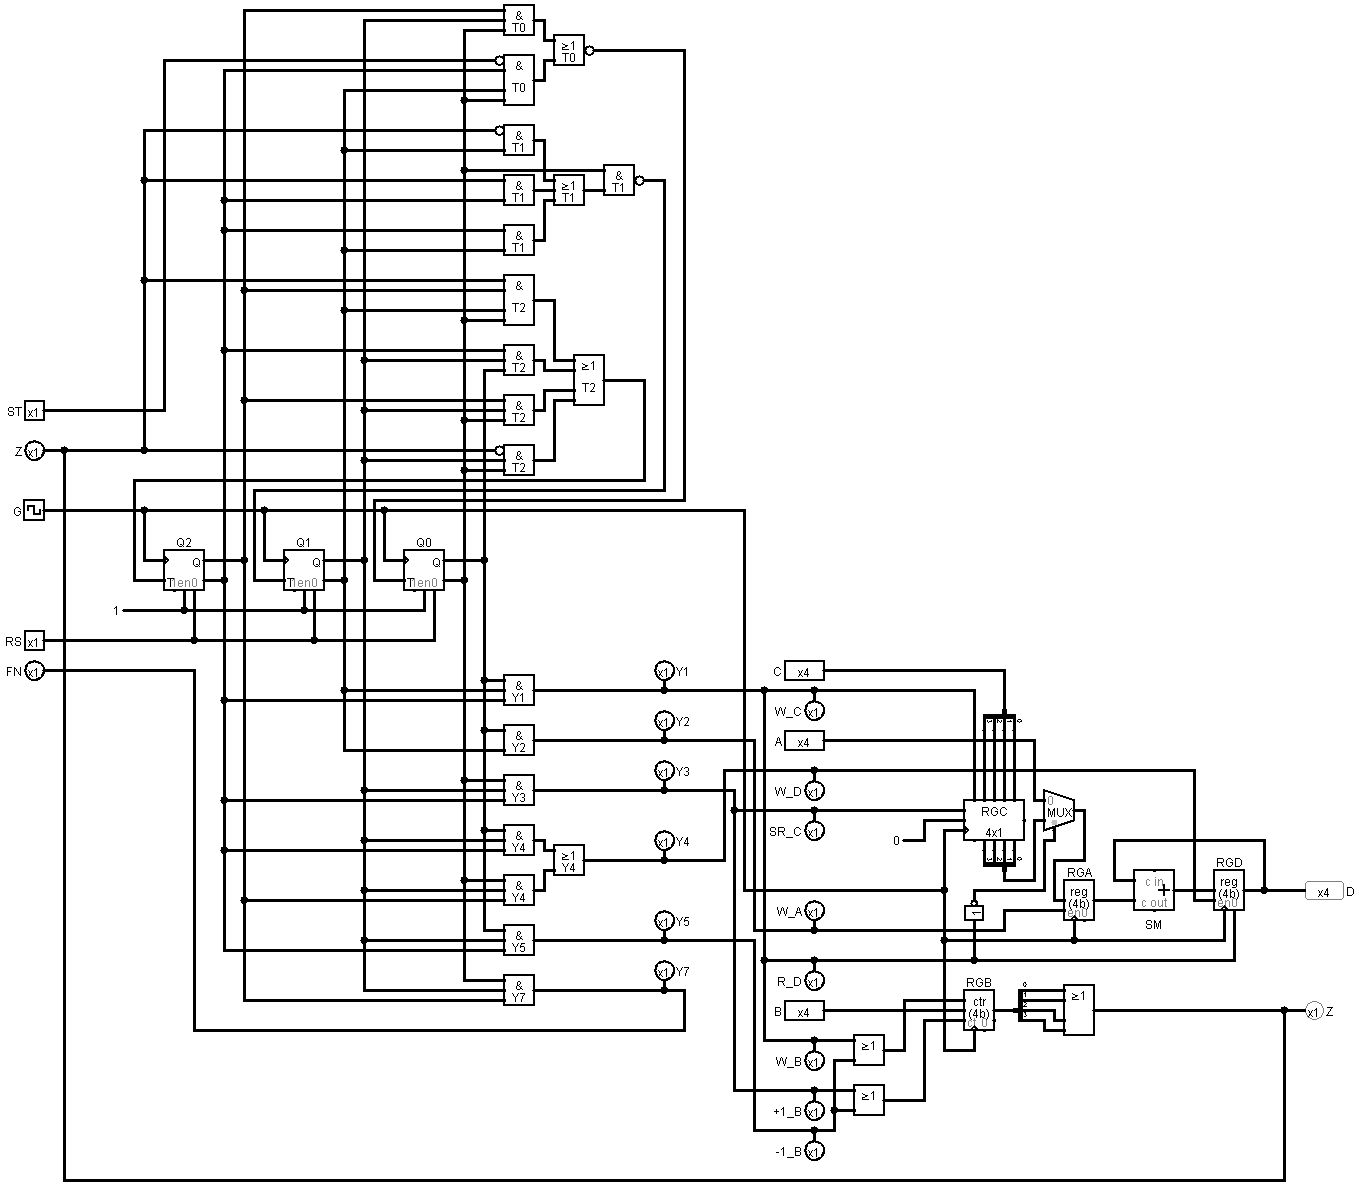
\includegraphics[scale=0.4, angle=90]{lab1.png}
\caption{Зiбрана схема.}
\end{center}
\end{figure}

\begin{table}[h!]
\centering
\begin{tabular}{|c|c|c|c|c|c|c|c|c|c|c|c|c|c|}
\hline
 G & ST & FN & RS & Z & $Q_2$ & $Q_1$ & $Q_0$ & $Y_1$ & $Y_2$ & $Y_3$ & $Y_4$ & $Y_5$ & $Y_7$\\
\hline
0 & 0 & 0 & 1 & 0 & 0 & 0 & 0 & 0 & 0 & 0 & 0 & 0 & 0\\
\hline
0 & 0 & 0 & 0 & 0 & 0 & 0 & 0 & 0 & 0 & 0 & 0 & 0 & 0\\
\hline
1 & 0 & 0 & 0 & 0 & 0 & 0 & 0 & 0 & 0 & 0 & 0 & 0 & 0\\
\hline
0 & 0 & 0 & 0 & 0 & 0 & 0 & 0 & 0 & 0 & 0 & 0 & 0 & 0\\
\hline
1 & 0 & 0 & 0 & 0 & 0 & 0 & 0 & 0 & 0 & 0 & 0 & 0 & 0\\
\hline
0 & 0 & 0 & 0 & 0 & 0 & 0 & 0 & 0 & 0 & 0 & 0 & 0 & 0\\
\hline
0 & 1 & 0 & 0 & 0 & 0 & 0 & 0 & 0 & 0 & 0 & 0 & 0 & 0\\
\hline
1 & 1 & 0 & 0 & 0 & 0 & 0 & 0 & 0 & 0 & 0 & 0 & 0 & 0\\
\hline
0 & 1 & 0 & 0 & 0 & 0 & 0 & 1 & 1 & 1 & 0 & 0 & 0 & 0\\
\hline
0 & 0 & 0 & 0 & 0 & 0 & 0 & 1 & 1 & 1 & 0 & 0 & 0 & 0\\
\hline
0 & 1 & 0 & 0 & 0 & 0 & 0 & 1 & 1 & 1 & 0 & 0 & 0 & 0\\
\hline
0 & 0 & 0 & 0 & 0 & 0 & 0 & 1 & 1 & 1 & 0 & 0 & 0 & 0\\
\hline
1 & 0 & 0 & 0 & 0 & 0 & 0 & 1 & 1 & 1 & 0 & 0 & 0 & 0\\
\hline
0 & 0 & 0 & 0 & 1 & 0 & 1 & 0 & 0 & 0 & 1 & 0 & 0 & 0\\
\hline
1 & 0 & 0 & 0 & 1 & 0 & 1 & 0 & 0 & 0 & 1 & 0 & 0 & 0\\
\hline
0 & 0 & 0 & 0 & 1 & 0 & 1 & 1 & 0 & 0 & 0 & 1 & 1 & 0\\
\hline
1 & 0 & 0 & 0 & 1 & 0 & 1 & 1 & 0 & 0 & 0 & 1 & 1 & 0\\
\hline
0 & 0 & 0 & 0 & 1 & 1 & 0 & 0 & 0 & 0 & 0 & 0 & 0 & 0\\
\hline
1 & 0 & 0 & 0 & 1 & 1 & 0 & 0 & 0 & 0 & 0 & 0 & 0 & 0\\
\hline
0 & 0 & 0 & 0 & 1 & 0 & 1 & 1 & 0 & 0 & 0 & 1 & 1 & 0\\
\hline
1 & 0 & 0 & 0 & 1 & 0 & 1 & 1 & 0 & 0 & 0 & 1 & 1 & 0\\
\hline
0 & 0 & 0 & 0 & 1 & 1 & 0 & 0 & 0 & 0 & 0 & 0 & 0 & 0\\
\hline
1 & 0 & 0 & 0 & 1 & 1 & 0 & 0 & 0 & 0 & 0 & 0 & 0 & 0\\
\hline
0 & 0 & 0 & 0 & 1 & 0 & 1 & 1 & 0 & 0 & 0 & 1 & 1 & 0\\
\hline
1 & 0 & 0 & 0 & 1 & 0 & 1 & 1 & 0 & 0 & 0 & 1 & 1 & 0\\
\hline
0 & 0 & 0 & 0 & 1 & 1 & 0 & 0 & 0 & 0 & 0 & 0 & 0 & 0\\
\hline
1 & 0 & 0 & 0 & 1 & 1 & 0 & 0 & 0 & 0 & 0 & 0 & 0 & 0\\
\hline
0 & 0 & 0 & 0 & 1 & 0 & 1 & 1 & 0 & 0 & 0 & 1 & 1 & 0\\
\hline
1 & 0 & 0 & 0 & 1 & 0 & 1 & 1 & 0 & 0 & 0 & 1 & 1 & 0\\
\hline
0 & 0 & 0 & 0 & 0 & 1 & 0 & 0 & 0 & 0 & 0 & 0 & 0 & 0\\
\hline
1 & 0 & 0 & 0 & 0 & 1 & 0 & 0 & 0 & 0 & 0 & 0 & 0 & 0\\
\hline
0 & 0 & 0 & 0 & 0 & 1 & 0 & 1 & 0 & 1 & 0 & 0 & 0 & 0\\
\hline
1 & 0 & 0 & 0 & 0 & 1 & 0 & 1 & 0 & 1 & 0 & 0 & 0 & 0\\
\hline
0 & 0 & 1 & 0 & 0 & 1 & 1 & 0 & 0 & 0 & 0 & 1 & 0 & 1\\
\hline
1 & 0 & 1 & 0 & 0 & 1 & 1 & 0 & 0 & 0 & 0 & 1 & 0 & 1\\
\hline
0 & 0 & 0 & 0 & 0 & 0 & 0 & 0 & 0 & 0 & 0 & 0 & 0 & 0\\
\hline
1 & 0 & 0 & 0 & 0 & 0 & 0 & 0 & 0 & 0 & 0 & 0 & 0 & 0\\
\hline
0 & 0 & 0 & 0 & 0 & 0 & 0 & 0 & 0 & 0 & 0 & 0 & 0 & 0\\
\hline
1 & 0 & 0 & 0 & 0 & 0 & 0 & 0 & 0 & 0 & 0 & 0 & 0 & 0\\
\hline
0 & 0 & 0 & 0 & 0 & 0 & 0 & 0 & 0 & 0 & 0 & 0 & 0 & 0\\
\hline
1 & 0 & 0 & 0 & 0 & 0 & 0 & 0 & 0 & 0 & 0 & 0 & 0 & 0\\
\hline
0 & 0 & 0 & 0 & 0 & 0 & 0 & 0 & 0 & 0 & 0 & 0 & 0 & 0\\
\hline
1 & 0 & 0 & 0 & 0 & 0 & 0 & 0 & 0 & 0 & 0 & 0 & 0 & 0\\
\hline
0 & 0 & 0 & 0 & 0 & 0 & 0 & 0 & 0 & 0 & 0 & 0 & 0 & 0\\
\hline
1 & 0 & 0 & 0 & 0 & 0 & 0 & 0 & 0 & 0 & 0 & 0 & 0 & 0\\
\hline
0 & 0 & 0 & 0 & 0 & 0 & 0 & 0 & 0 & 0 & 0 & 0 & 0 & 0\\
\hline
\end{tabular}
\caption{Часова діаграма.}
\end{table}
\end{document}
